\documentclass{article}
\usepackage[utf8]{inputenc}
\usepackage{tikz}
\usepackage{standalone}
\usepackage{amsmath}
\usepackage{amsfonts}
\usepackage[a4paper,margin=3cm]{geometry}



\title{Causal Effect Inference with Normalizing Flows}
\author{Micha de Groot}
\date{August 2019}

\begin{document}
\maketitle

\noindent
The goal of this project is to see if it is possible to extent the work of Louizos et al. \cite{louizos2017causal} through the use of Normalising Flows. Louizos et al. have shown that variational inference can be used for causal inference. We now want to discover if we can improve of their VAE-based \cite{kingma2013auto} method with Normalising Flows \cite{rezende2016variational}\cite{berg2018sylvester}\cite{dinh2016density}. It has been shown that these models are capable of capturing more diverse and complex posterior distributions, which is needed in this research.

The first phase of the project directly extends the causal VAE to a causal VAE with Normalising Flow. We hypothesise that this works slightly better because the model can capture a more complex latent distribution. Though a limitation here is the complexity of the dataset and the causal effect that we want to model. The commonly used datasets in causal inference all have a binary, one-dimensional treatment or intervention variable and a one-dimensional scalar as outcome variable. The observed feature vectors are, by deep learning standards, very low dimensional. This all means that the potential modelling power that Normalising Flows possess probably won't reach their full potential. 

To display this full modelling power we are going to generalise the problem in the second phase. This will be split into different components and will likely be the core of the project.

\section{Directions in which we want to generalise the model}
Several steps that we want to take to generalise the problem
\begin{itemize}
    \item Step away from the assumption that the treatment is binary and one dimensional. We either make the treatment variable categorical or continuous. It also has to be higher dimensional, maybe in such a way that it can't be directly interpreted.
    \item Learn the intervention. In the original model all possible values of the intervention are known and seen during training. We want the model to learn the general concept of the intervention variable and being able to handle intervention samples that are (slightly) different from the ones in the training set.
    \item It is important in all these extensions that it shouldn't suffice to learn correlations between variables. It has to be the case that there is a causal effect with some form of latent confounding.
\end{itemize}


% \section{Learn the intervention}
% Don't assume that we (can) know all the values the intervention can take. Combine learning the outcome for a given intervention with learning what intervention will yield a <high> outcome.

% What is important to note here is that we are not necessarily looking for a model that takes good actions, but one that learns the causal effect of certain interventions. The novelty would be that the model could generalise to interventions that it hasn't seen before.

% \subsection{Construct a scenario where you really have to learn cause and effect}
% Some scenarios that could be predicted with our model could probably also be predicted with a model that learns correlations between the values of interventions, outcomes and features.

\section{New idea}
We need a problem where there is an effect of one variable $t$ on another variable $y$. We need to be able to observe both, but their dimensions might be entangled in some way. It could help if there is more information we can observe, $x$, that tells us more about a possible latent representation of the current sample/state. There \textbf{has} to be latent confounding between $t$, $y$ and $x$. Otherwise we could directly estimate covariates for $t$ and $y$ from $x$ without the need to model any latent variables/confounders. 

What is preferable is that the observed variables have a reasonable high dimensionality. For $t$ and $y$ that means at least three dimensions. For $x$ at least one hundred. An obvious direction for this would be to have images as our observed variables. Firstly this makes for a cooler presentation at the end, and secondly because there are no SOTA methods that can work with raw images that don't use any form of deep learning. This also makes the need for Normalising Flows more apparent because images have a complex distribution.

Now the question is: what can be the outcome variable in an image and what can be the intervention? We could have as input one image, $x$, an outcome image $y$ and an intervention $t$. Then it has to be the case that there always is a difference between $x$ and $y$ even if the intervention is zero. That would make it so that there is a difference between $x$ and $y$ that is partially caused by $t$ and partially caused by $z$, who's posterior we would estimate from $x$. It also has to be the case that $x$ is actually caused by $z$, but that can be arranged if we generate the images ourselves. 

%What would we actually measure in this setup? The modelling of the intervention or the modelling of the outcome or both?

\subsection{Dataset idea}
We have an image $x$, that contains a shape, let's say a circle. It also contains an arrow (?) or other visual clue about what the intervention will be, or no clue if there is no intervention. The outcome $y$ is always different from $x$ to make sure there is confounding between the intervention and the outcome. But this difference is always independent of the intervention. Then the model has to reconstruct $x$ back from the latent space, learn what the intervention clue $t$ means and what the outcome $y$ will be after the intervention. The intervention can be that the shape has moved in the direction of the arrow for instance. The effect from $z$ on $y$ can also be a translation, or a linear transformation.

To actually know if the model has disentangled the shape from the intervention we can hold out something from the training set. We can either change the shape to a new one, given that the model has seen a variety of shapes, or we can only show arrows with a range of $-\pi/2$ to $\pi/2$ during training and show all possible angles/more angles during test time.

The difficulty of this setup can gradually scaled up to contain either more shapes, objects colours, intervention types or any combination of the previous. If all these setups show that the model is capable of learning the intervention effect we could transition to frames from a 3D environment.

All of this would require CNNs. What we don't know yet is if it would require flow-based models as well. In a way it makes sense that the latent representation $z$ would become too complex to capture if it has to encode both the object in the image as well as the intervention. 

Does this translate in any way to a real world problem? Well the model has to learn specifically what the intervention changes about the image, and thus about environment. It seems similar to a form of disentanglement so we have to figure out if this hasn't been done before.

During training the input would be $x$. The model has to estimate $z$, from that reconstruct $x$, infer $t$ and infer $y$. All three observed variables are used as labels when calculating the loss even though only $x$ is given as input. during test time we would show the model a new $x$ and let it estimate $z$. We can then let it infer $t$ and then $y$, or we could do an actual intervention by setting $t$ to a specific value ourselves and let it infer $y$ with the intervention value of $t$.

% If we would do an actual intervention and change the value of $t$, do we then change the value of $p(t|z)$ to $\delta(t)$ in the decoder? Yes, during training we have the real values of $t$ so we can force the model to learn a specific representation of $t$. But is it  realistic in a real-world scenario that we know the value of $t$? Yes but only certain ones for the events that we actually observed.

% Maybe we can also learn the model the concept of a translation and then let it translate an object by an unknown distance.

% Now that I think about it this seems similar to what Pim did. Except that in his case the model had to choose an action, which was the intervention variable. 

% \subsection{Dataset idea 2}
% Can we expand on the previous idea by adding some complexity? Now we just have one object and another object that is the intervention. Maybe a view form some 3D environment? Or $x$ could just have a far more complex pattern, but the intervention is still a rotation of everything. The intervention could also be more complex. The previous idea is mostly a translation or rotation. We also might have to be wary that the input of the encoder isn't just a concatenation of two images, one with $x$ on it and one with $t$ on it.

% A possibility to increase the difficulty of the problem is by making a possible intervention do two 'things', or by having multiple objects in the image. We could for instance have an intervention that causes the/a blue object to be translated and the/a red object to be rotated. Then we could have the model learn that if a certain colour object is not in the image it shouldn't do anything.

\subsection{Metrics}
What would we define a success in this task? Of course we want a good ELBO but that shouldn't be the goal. If we focus on learning the intervention we want to have some ground truth of $y$ and $t$. Is that different than just the reconstruction loss of $t$ and $y$? We're not necessarily interested in the best reconstruction of $y$ but in the state of the object in the image on which the intervention was applied. We do have a ground truth of the parameters of each object in the image so we could calculate Intersection over Union for example.
\newpage
\subsection{Example what the data will look like}
\begin{figure}
    \centering
    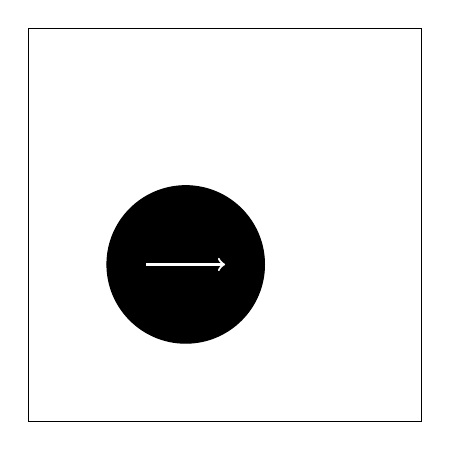
\begin{tikzpicture}
    \draw[](0.0, 0.0) rectangle (5.0, 5.0);
    \draw[fill=black] (2.0, 2.0) circle (1cm);
    \draw[->, draw=white, thick] (1.5, 2.0) -- (2.5, 2.0);
\end{tikzpicture}
\quad
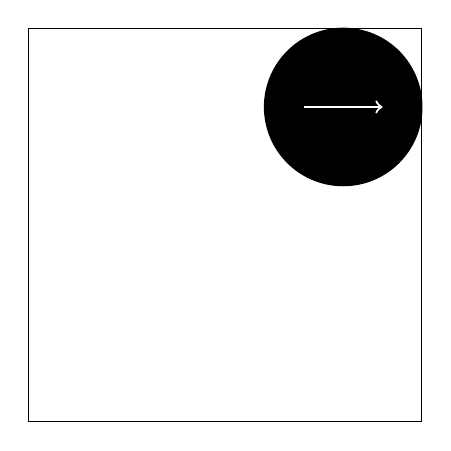
\begin{tikzpicture}
    \draw[](0.0, 0.0) rectangle (5.0, 5.0);
    \draw[fill=black] (4.0, 4.0) circle (1cm);
    \draw[->, draw=white, thick] (3.5, 4.0) -- (4.5, 4.0);
\end{tikzpicture}
    \caption{Example of a data sample. Left hand side is $x$, right hand side is $y$.}
    \label{fig:my_label}
\end{figure}
 The figure above gives an example of the most simple version of the problem. The real, disentangled $z$ value would in this case be a 6-D vector. It contains the coordinates of $x:(2,2)$, relative translation caused by the intervention $t: (2, 0)$ and translation that is applied to $x$ if $t$ was a zero-vector: $(0, 2)$. The model has to learn that this specific arrow causes the circle to translate two cm to the right and that the circle will always move two cm to the top. In this example the function that goes from $z$ to $t$ is just the identity, but it could also be that this arrow, with latent code $(2, 0)$ means that the intervention $t$ would be: cause the object to be blue.  To intervene in this example during test time we manually change the 2-D value of $t$. Disentanglement of $z$ should not be needed as we learn a function that infers the parameters of $t$ from $z$.



\subsection{Approach}
To solve this problem several steps need to be taken:
\begin{itemize}
    \item Define exact structure of the dataset and interventions
    \item Generate a dataset with a clear difference between the train and test set
    \item Choose and implement appropriate NF model
    \item Rewire the existing model somewhat to be able to handle this problem
    \item Train the NF version and the VAE version
    \item test interventions on both models
    \item Make qualitative analysis of results/reconstructions on the test set
\end{itemize}

\bibliography{references.bib}
\bibliographystyle{abbrv}

\end{document}
